\documentclass{article}
\usepackage[utf8]{inputenc}
\usepackage{amsmath}
\usepackage{amssymb}
\usepackage{hyperref}
\usepackage[normalem]{ulem}
\usepackage[numbers]{natbib}
\usepackage[colorinlistoftodos]{todonotes}
\usepackage{booktabs}

%\usepackage[colorlinks=true, allcolors=blue]{hyperref}

\usepackage{pifont}% http://ctan.org/pkg/pifont
\newcommand{\cmark}{\ding{51}}%
\newcommand{\xmark}{\ding{55}}%


\title{VAE Cookbook: \\its why and how, and the recent advances}

\setlength{\parskip}{\baselineskip}
\setlength{\parindent}{0pt}



\newcommand{\R}{\mathbb{R}}
\newcommand{\D}{\mathcal{D}}
\newcommand{\X}{\mathcal{X}}
\newcommand{\Y}{\mathcal{Y}}
\newcommand{\h}{h}
\newcommand{\N}{\mathcal{N}}	
\newcommand{\E}{\mathbb{E}}
\newcommand{\ELBO}{\mathcal{L}}

\newcommand{\prob}[3]{{#1}_{#2} \left( #3 \right)}
\newcommand{\condprob}[4]{{#1}_{#2} \left( #3 \middle| #4 \right)}
\newcommand{\expected}[2]{\mathbb{E}_{#1}\left[ #2 \right]}
\newcommand{\KL}[2]{D_{\mathrm{KL}}\left( #1 \| #2 \right)}

\newcommand{\pp}{\theta}
\newcommand{\x}{\mathbf{x}}
\newcommand{\z}{\mathbf{z}}
\newcommand{\layers}{L}


\newcommand{\dimpp}{D}

\begin{document}
\maketitle


\tableofcontents
\newpage



\section{Overview}

Deep generative models are popular nowadays when used for unsupervised learning and for modeling structured outputs.
In both cases, the variable that one wants to model contains some structure that cannot be modeled simply via describing its lower order moment or linear correlation. 
Examples include natural images, natural languages, audio data, etc.

There exists many ways to model the structure of a multivariate distribution, such as (1) autoregressive models which assume the joint probability of the random variables can be factorized as a product of distributions, (2) energy-based model that define the interaction, or compatibility between the values of the random variables, and (3) latent-variable models \todo{link to VLM page} that assume there exists an unobserved latent variate which can often be thought of as a lower dimensional representation of the data.
We focus on the last category in this monograph, as for the problems that we are going to visit it is a natural assumption to make.

Specifically, the Variational Autoencoders introduced by \citet{kingma2013auto} assumes a continuous latent variable model, with a Gaussian prior in the latent space. 
It is a reasonable assumption to make in many cases, such as for visual imagery: when we move the latent representation of an image in the vicinity of the latent space, it corresponds to changes in shape, color, intensity of light, location of an object, or different kinds of high level semantics of the image. 

However, training deep continuous latent variable models with nonlinear mapping between the latent code and the observed variable was not so successful only until recently.
This is because evaluating the likelihood of a data instance relies on inferring the latent representation, and for non-linear, non-conjugate prior-likelihood pair inference cannot be conducted exactly, or in a computationally tractable way. 
So we need to \textit{approximately} infer the latent representation.
We will talk more about this in [\todo{EM and ELBO}].

We rely heavily on a family of approximate inference techniques known as the \textit{Variational Inference} (VI), which is to cast the inference process as an optimization problem by dealing with a lower or upper bound on the original objective. 
This is different from the sampling-based \textit{Markov Chain Monte Carlo} (MCMC) methods in many ways. 
One important aspect is the \textit{bias-and-variance} trade-off underlying these two classes of algorithms. 
The MCMC methods often result in high variance estimates but are asymptotically unbiased, while the VI methods have lower variance but due to its choice of (often well-understood and tractable) variational family of distributions are often biased. 
Even though the variational methods are known to have lower variance, the gradient estimate needed for updating the parameters during training can be very noisy, due to the intractable VI objective that can only be optimized via stochastic gradient methods. 
We will extend the discussion of this perspective more in [\todo{variance reduction}].



The goal of this monograph is to cover the (1) necessary background to understand latent variable models and its training, different views on the well-known variational autoencoders: both (2) from the generative model point of view and (3) from the information theoretic point of view. 
We will also cover the (4) the intuition of optimizing the objective, (5) training details, and (6) different ways to improve the model, with a hope to help deep learning researchers to better understand the probabilistic aspect of deep generative models and how to use them as a tool. \todo{CW: these correspond to item 1-6 in the list below}





LINKS (navigating page)
\begin{enumerate}
\item Latent Variable Models
\item Training: the Evidence Lower Bound
\item Information theoretic intuition of the ELBO
\item Autoencoders as generative models
\item The double-edged sword: $\KL{q}{p}$
\item Improving the models: the Holy Trinity
\item Evaluation
\item Variance reduction
\end{enumerate}





\todo{[CW] overall missing: DRAW, variational memory models (few shot generation), variational addressing, beta-VAE, over-pruning problem, discrete LVM}


\section{Some background stuff}

\subsection{Maximum likelihood principle}

When we have a model $p_\theta$, the likelihood of the data sampled from the true data distribution $p_\D$ tells us how good our model is. 
We write it as $\E_{p_\D}[\log p_\theta(x)]$, where the subscript $\theta$ is the parameters of our model.
$\theta$ is the sufficient statistics of our model, which can be thought of as a summary of the distribution; i.e. the mean and variance of a Gaussian distribution.

In plain language, the Maximum Likelihood Principle in order to make our model a better model, we need to adapt it to make it seem more like the distribution that the data is sampled from.
This is to find the values of the model parameter $\theta$ that maximizes the likelihood function.
Most of the time the true data distribution is not available, so we would instead have access to an empirical distribution which we call the training set.
Suppose we have $n$ i.i.d. samples, so the likelihood of this training data can be written as a sum of $n$ terms; the \textit{maximum likelihood estimate} (MLE) is 
$$\theta^* \in \{\underset{\theta}{\textnormal{argmax}} \sum_{i=1}^n\log p(x_n)\} $$


So far we have been talking about the case of a single random variable.
The same principle can be extended to 



- what is maximum likelihood, maximum conditional likelihood, and maximum joint likelihood. 

\subsection{Marginal likelihood}

- In the face of partial observability ...

- max complete data log likelihood





\section{Variational Autoencoders:\\Not just an autoencoder.}


%In fact, not really an autoencoder either \citep{chen2016variational}.

\todo{rewrite "Autoencoders as generative models"}
\todo{talk about amortized inference -> introduce the concept of encoder}
\todo{intuition of how an autoencoder can be thought of as a generative model}
\todo{"Not just an autoencoder." can be another sub-section -> lossy encoding? hierarchy of representations}


In the long history of research into artificial neural networks, autoencoders are an interesting topic. The autoencoder is trained to be an identity 


They are commonly used to learn an encoding of the input. Most use a dimension bottleneck in the hidden layers to achieve a non-linear dimension reduction, but it is also sometimes useful to use a higher dimension, like in sparse autoencoders. During the resurgence of neural networks as deep learning, autoencoders were largely used to do pretraining.
\citep{bengio2013generalized} first interprets a special kind of autoencoder, called the denoising autoencoders, as a generative model. 
One connection to make is that in their work, an unstructured noise is injected to the data, 

The introduction of VAEs \citep{kingma2013auto} interprets the autoencoder as a graphical model with the encoding being a latent variable to be inferred. While autoencoders on their own weren’t a probabilistic model before, the VAE framework offers an alternative look at them as such. 

Because they were introduced as a generative model, one of the more common applications of VAEs is to generate images, i.e: sampling from a Gaussian distribution and pushing that through the decoder. Another application of VAEs are what autoencoders were used for before: learning non-linear representations of the input.

However, the framework VAEs introduce is capable of much more. 
In DeepMind's paper on the topic, they refer to these models as Deep Latent Gaussian Models (DLGMs) \citep{rezende2014stochastic}. 
We think this may be more descriptive, although we need not limit ourselves to Gaussian distributions. 
Sure, you \emph{can} use VAEs to autoencode, but using them for just that is missing the point \cite{chen2016variational}.


\todo[inline, color=green!40]{Explain how to improve}


Thus far, VAEs have been used to:
\begin{itemize}
\item Isolate known factors from unknown factors causing the observed data: e.g. \cite{kingma2014semi}.
\item Disentangling (to some extent) unknown factors causing the observed data: e.g. \cite{higgins2016beta}.
\item Leveraging bigger datasets to achieve meta-learning on a smaller set of data:  e.g. \cite{edwards2016towards}
\end{itemize}%CW: citations?

%In this article, we hope to introduce you to the benefits of modelling your data with latent variables, and suggest simple recipes to use VAEs in your work. %\todo{CW: what recipes exactly (motivation, intuition, wide but not exhaustive summary of the literature)}




\section{Latent Variable Models: What is it good for?
}

Deep neural networks (DNN) have been shown to be a powerful inference tool in multiple domains in recent years. 
%Its success can be attributed to, but is not limited to, the expressiveness of the network itself, optimization and regularization effect of training with stochastic methods. 
Its expressiveness allows one to take the available information to answer a question of interest. 
%The convenience of training a model from one end to another 
For example, given someone's occupation and age, we can predict his salary. 
Given a patient's X-ray image, we want to determine whether he has cancer. 
Or by giving the computer a set of images, we can ask it which of them are dogs and which of them are cats, which is one of the popular tasks in machine learning.

\subparagraph{Representation and Modeling.} 
The problems above can all be formulated as a conditional probability of a pair of variables $(X,Y)$, e.g. $X$ being X-ray images and $Y$ being a Bernoulli variable: $1$ if someone has cancer and $0$ if not. 
Here we are simply interested in $p(Y|X)$. 
As stated, DNNs are powerful tools to model this kind of conditional probabilities because of its expressiveness and the simplicity in thinking about the conditional relationship.
But can we do more?

Lets think about the case where we only observe variable $X$, which denotes one's salary. 
In our belief, there is a latent state $z$ associated with each instantiation, $x$, of the observed variable $X$.
Modeling this latent variable along with the observed variable allows us to better capture the characteristics of the unknown distribution of interest. 
For instance, the true income distribution might have multiple modes. 
We thus assume the prior distribution $p(z)$ to be a multinoulli distribution; each $z$ can take on one of the three indices $\{0,1,2\}$ denoting low, average and high income groups. 
In some simple cases, one can infer the posterior probability $p(z|x)$ (in exact form), which in our example means the probability of someone falling in one of these groups given his salary information.

What if we want to model more complicated relationships between latent states and observable attributes? 
Take natural images for example. 
One might want the latent state to encapsulate some ``semantic'' information of an image, such as the identity of a person in the image, whether someone is smiling and wearing glasses, if there's a cat or dog in the image, etc. 
On the other hand, there might be different levels of factors that result in the image we now see, including lighting, angle, whether the lens of the camera is clean or not, and a lot of other variations. 
With slight abuse of language, we refer to all of these unobserved factors that are correlated with the observed variable as latent state. 
We are now interested in modeling the complicated mapping from the latent state to the observed variable, and naturally choose to use DNNs to define such a mapping.
This is also known as deep latent variable models, or \href{http://videolectures.net/deeplearning2017_welling_inference/}{\emph{deepification}} of latent variable models (LVM).

\subparagraph{Limited and Incomplete Data.} 
Another usage of LVM is to deal with the scarcity of the data. 

When data instances are lacking, it will be better to leverage prior knowledge on functions into modeling, to prevent overfitting or help the model generalize better. 
Such approaches stem from the Bayesian community and have gained tremendous popularity when combined with Deep Learning techniques. %cite BDL workshop, YWT's nips talk?
Treating weights of a DNN as a random variable, for instance, allows us to calibrate predictive uncertainty, by sampling i.i.d. samples of weights from the so-called posterior distribution. 
The posterior predictive is better calibrated since making a prediction requires averaging over multiple samples of weights, which gives it an \textit{ensemble} interpretation. 
Think of each sample as an expert, who has its own knowledge about how to capture the correlation among the variables (e.g. $Y|X$). 
All the experts need to reach a consensus for the posterior predictive to express high confidence in one prediction; otherwise the great dispersion of the posterior predictive can serve as a warning for one not to trust the model!

Another kind of scarcity is the incompleteness of data features. 
For example, the latent state examples above all fall into this category, as we can think of the unobserved variables (semantics, lighting variations, modal characteristics of the data distribution) as features that are never provided, thus always incomplete.
%Training a deep LVM has the benefits of either better interpretability or leveraging statistical strength when the model is better structured.
%Below we discuss a suite of examples of training a deep LVM with the benefits of either better interpretability or leveraging statistical strength when the model is better structured.

In machine learning problems, we often represent our data in tensor form. 
In 2D cases, we consider a dataset matrix; the number of rows ($N$) corresponds to the number of data samples and the number of columns ($M$) corresponds to the number of features.
When $N$ is small, then we don't have enough data instances and when $M$ is smaller than we believe, there are some features that are unobserved. 
These are the two general cases that are just discussed above. 
We can also represent the dataset in higher dimensional tensor or a graph, and there are other kinds of incompleteness, such as views, labels, etc.
Below, we discuss some more applications of deep LVM and try to connect to the perspective of scarcity. 




\subsection{Applications of Deep Latent Variable Models}

\subparagraph{Semisupervised Classification.}
% talk about introducing y as partially observed variable, class and style
Lets turn to our all time favorite dataset, the MNIST hand-written digit. 
The dataset comes in image-label ($x$-$y$) pairs. 
We'd like to create a semi-supervised scenario where the labels are only partially observed: sometimes you have them, sometimes you don't.


\citet{kingma2014semi, maaloe2016auxiliary} introduce a way to model partially labeled data with variational autoencoders. 
The idea is to build a LVM on the images ($\x$). 
Remember that the latent state of the observed images can be used to model high level semantics, low level variations and the modal characteristics of the data distribution. 
Here we want to separate the digit's class ($y$) from other variation ($\z$), such as style, orientation, and the thickness of the brush. \todo{figure}
In the generative process, given the class of the digit $y=j$, the digit is generated from the latent state that is sampled independently from a prior of all the other variation $x\sim p(x|z,y)$ and $z\sim p(z)$.
For data points that are labeled, we infer the latent state $z$ as usual for training (which we describe below), and for data points that are not labeled with classes, naturally, the thing to do is to marginalize over all possible labels. 
In plain words, lets assume we are given a classifier of digit classes $q(y|x)$, which can be trained jointly on labeled data. 
We need to consider all possible classes of a certain image ($i$), which has probability $p(y_i=j|x_i)$, and maximize the likelihood of the data point being in that class.

This approach allows us to treat the regressand as a latent variable and train the joint probability generatively when labels are not provided (incomplete data), and train the inference model/classifier discriminatively when labels are given. 


%In this scenario, since there are only 10 digits, this is possible. When the number of classes gets large, perhaps sampling might be in order. However, there are tradeoffs involved when dealing with discrete variables, for more information see the subsection about discrete variables.



\subparagraph{Unobserved Confounders.}
% talk about socio-econo and confounder 
To analyze the effect of an independent variable $x$ on the dependent variable $y$, sometimes we need to suppress the ``confounding" effect of an extraneous variable $z$ that influences both $x$ and $y$. 
The variable $z$ is known as the confounder of the causal relationship between $x$ and $y$. 
Consider $x$ to be whether a Facebook post is associated with an image, a selfie for example, or not, and $y$ to be the number of likes it has. 
We now want to know whether taking a selfie while posting something has a positive effect on the number of likes the post can get. 
If we simply collect data from the general public, we will also need to take how popular and how outgoing someone is into account, which has an influence on whether his or her posts usually come with a selfie and on the number of likes he or she can get. 

Another interesting example is given by ~\citet{louizos2017causal}.
In this paper, they treat the confounder $z$ as a latent variable, as a confounder is usually not observed (again, incomplete data). 
The confounder (such as one's socio-econo status) has a direct effect on the intervention $x$, such as the medication a patient has access to, and the outcome $y$, such as the patient's health condition.
Without measuring the confounder, there's no general way to isolate the causal effect of medication on the patient's health. 
They propose to incorporate a noisy view $v$ on the latent confounder, for example the patient's income, that is highly correlated with the latent confounder.
The observed confounder thus can be used to infer the latent confounder and allow us to inspect individual causal effects.

\subparagraph{High-Level Semantics.}
% talk about pixelvae and vlae (mention ladder first), generating sentences from cont space
% not exactly an autoencoder
% disentanglement
\begin{figure}
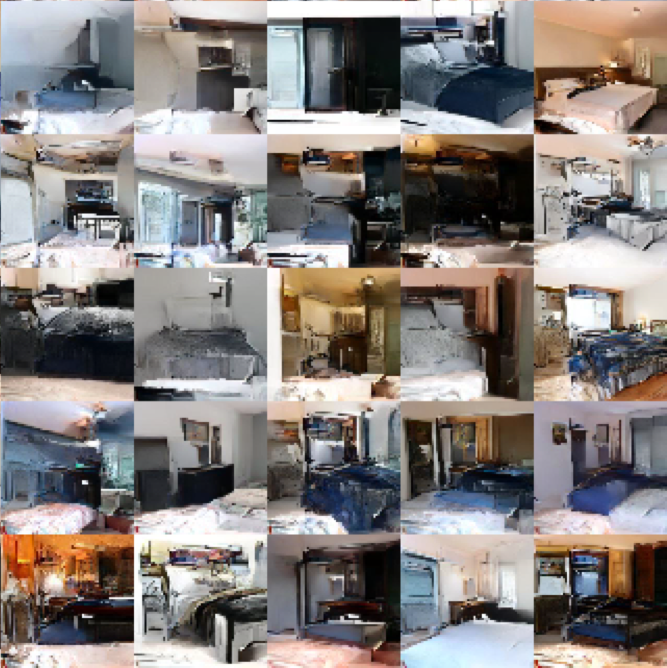
\includegraphics[width=0.32\textwidth]{figures/pixelvae_z2.png}
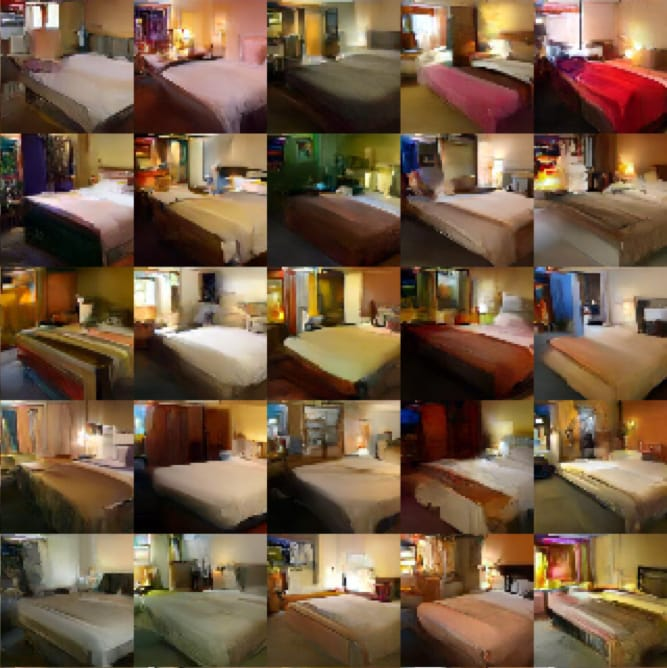
\includegraphics[width=0.32\textwidth]{figures/pixelvae_z1.jpg}
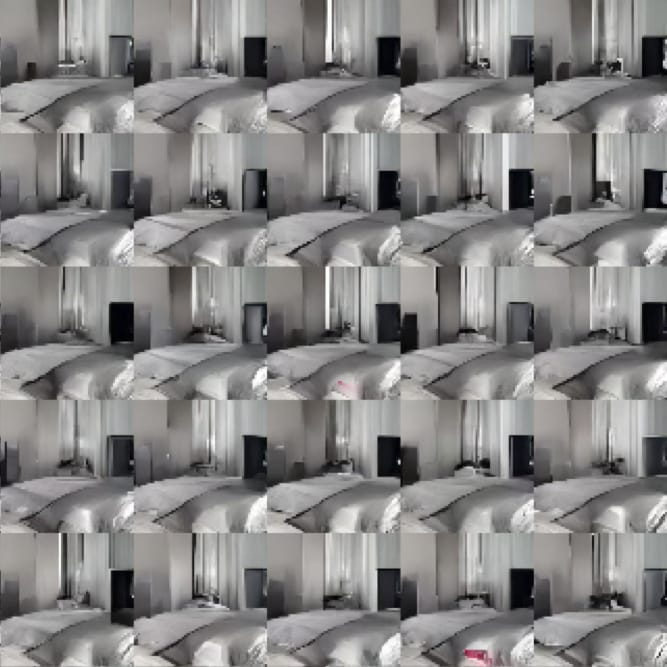
\includegraphics[width=0.32\textwidth]{figures/pixelvae_x.jpg}
\label{ref:pixelvae_difflayers}
\caption{Variation in different levels of a kind of hierarchical VAE called PixelVAE \cite{gulrajani2016pixelvae} (with autoregressive likelihood instead of conditionally independent distribution such as fully factorized Gaussian). The samples are generated by sampling from certain layer while holding the others fixed as deterministic hidden units (taking only the mean of a Gaussian). Left: {Sampling from the top level layer ($z_2$)}, Middle: {Sampling from the middle layer ($z_1$)}, Right: {Sampling only from the pixel level ($x$)}.}
\end{figure}
Extracting different levels of representation of the data is a fundamental problem of deep learning. 
The aim of an autoencoder is to learn a meaningful encoding of the data that can be used to reconstruct the original data points.
Through reconstruction, the structure in the original data distribution is recovered. 
This is done by mapping from the representation, or the code, through the decoder which defines the structure, i.e. the information that is lost during encoding. 
By imposing a ``simple'' prior distribution on the latent representation, we hope the encoder will destroy such structure in the data distribution and rely on the decoder to ``semanticate'' the unstructured codes. 
It is also possible to gradually remove the structure to have a hierarchy of representations. \todo{CW: trim this...}

Assuming a hierarchy of latent states allows us to do this. 
Consider the following generative model, in which the latent variables $z$ are split into $L$ layers:
\begin{equation}
p(x,z) = p(x|z_1)p(z_L)\prod_{l=1}^{L-1}p(z_l|z_{>l})
\end{equation}

This allows us to model different layers of latent representations.
At the top layer, high level information that everything else depends on is represented. 
For instance, if the model knows the image has a frog in it (conditioned on $z_L$ being equal to or close to some vector representation of a frog), the lower level representation could be natural scenes such as a pond, magnolia leaves or insects that are highly correlated with a frog in an image. 

\citet{sonderby2016ladder} is one of the first papers that build on hierarchical VAEs, followed by \citet{gulrajani2016pixelvae} and \citet{chen2016variational}.  
In the latter two, the authors proposed to use an autoregressive decoder called PixelCNN \cite{oord2016pixel} to model the low level correlation between the pixels. 
This helps to separate high level semantics from the textural details of the image.
See Figure \ref{ref:pixelvae_difflayers} for an illustration.
The same idea was explored independently by \citet{agrawal2016deep} using RealNVP \cite{dinh2016density} to make the adjacent pixels dependent on each other given the latent state. 
Another line of research focusing on adversariallly trained inference \cite{dumoulin2016adversarially} mechanism has also been exploring the hierarchical representations of data \cite{anom2017hali}. 
Finally, \citet{bowman2015generating} tried to explore the same idea with language, hoping to separate semantics of a sentence from its syntax which can be modeled by a conditional language model (such as an RNN). 
\todo{cW: beta-VAE (disentanglement)? maybe somewhere else ...}



% LVAE
% pixvae + VLAE (gulrajani2016pixelvae, chen2016variational)
% VAE + language model (bowman2015generating)
% VAE + RNVP (agrawal2016deep)
% beta-vae?


%\subparagraph{Conceptual compression.}
% conceptual compression (not necessary more interpretable, but shorter code, link to disentanglement below) 

\subparagraph{Neural Statistician.} Earlier we talked about treating parameters of a model as random variables, and since it is not observed, we need to infer it based on the observations, in this case the whole training data. 
Lets denote these stochastic parameters as $c$, and we are interested in inferring the most likely $c$ given $\mathcal{D}$, i.e. $p(c|\mathcal{D})$.
Carrying on the terminology of deep LVM, $c$ is the latent state of $\mathcal{D}$, which is now not an observation of a single data point but the whole set of training data.

[cont'd]


% [towards a neural stats]
% [deep prior]

%Probabilistic models allow one to assume conditional dependencies among random variables, which provides a way to 




%%%%%%%%%%%%%%%NOTES%%%%%%%%%%%%%%


%Inference (take available information and conclude) -> direct inference (prediction) -> inferring unknown -> latent variable examples

%Why do we care about latent variables? (limited data view: limited instances and limited observable features) (structured probabilistic models: interpretability and imposing prior knowledge)

%A suite of examples 
%Deepification (non-linear relationship)

%Likelihood, latent variable models, autoencoding variational bayes



\section{Two Views of the Variational Lower Bound}


% https://en.wikipedia.org/wiki/Variational_Bayesian_methods

\subsection{Information-theoretic (intuitive)}

\begin{figure}
\begin{center}
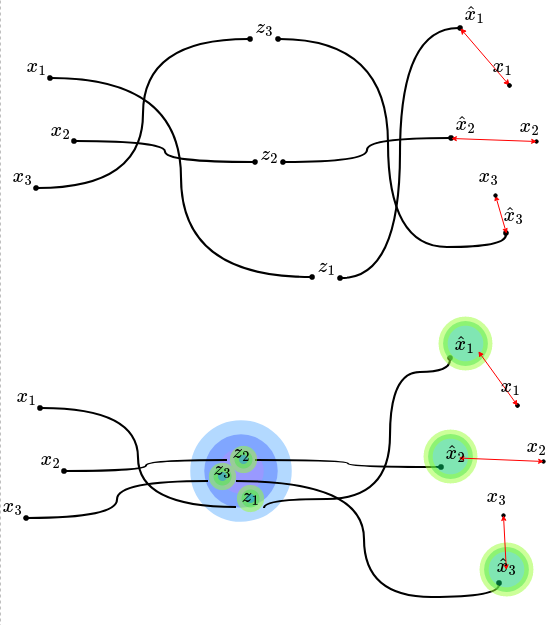
\includegraphics[width=0.75\textwidth]{figures/autoencoder_vs_vae.png}
\end{center}
\label{fig:ae_vs_vae}
\caption{Above: A standard autoencoder, which maps from the $x$ space to the $z$ space, and then maps that back with a reconstruction term depicted in red. Below: The variational autoencoder maps from $x$ to a \emph{distribution} over $z$, with a KL-divergence term over the approximate posterior (green) and the prior distribution (blue), which can be seen a regulariser.}
\end{figure}
For this view, we are trying to minimise the following objective:
$$\underbrace{-\expected{\condprob{q}{}{\z}{\x}}{\log \condprob{p}{}{\x}{\z}}}_\text{
 Reconstruction loss}
+ \underbrace{\KL{\condprob{q}{}{\z}{\x}}{\log \prob{p}{}{\z}}}_\text{
 Information gain
}$$
which is the standard VAE loss to \emph{minimise}.

Karol Gregor explains VAEs in \href{https://youtu.be/P78QYjWh5sM?t=207}{this lecture}. At the timestamp, he talks about an information-theoretic interpretation of the VAE loss. From this perspective, the KL-divergence term is viewed as an information bottleneck: The objective is to reconstruct the input while transmitting as little information as possible from the encoder to the decoder.


Thinking of the KL-divergence term as a regulariser allows us to relate it back to things like sparse autoencoders or contractive autoencoders. The reconstruction term is balanced with a regularisation term on the hidden representation. In a standard autoencoder, the encoder maps $\x$ to the hidden representation deterministically, with no constraints. The decoder then maps this representation back to the original input. In VAEs, the KL-divergence term regularises this representation $\z$ so that in aggregate, they form a Gaussian distribution. See Figure \ref{fig:ae_vs_vae}. This then allows you to sample from the prior $\prob{p}{}{\z}$ which is a Gaussian to generate images similar to your data.


However, one misunderstanding about the KL-divergence term is that it should be close to 0 for a good model. What this interpretation tells us that this shouldn’t be the case: a KL-divergence term close to 0 means no information is being transmitted by the encoder to the decoder. In our running example about salaries, knowing someone's salary should narrow down which group he belongs to, giving us some \emph{information} about $\z$.

The great thing about looking at it this way is that you can think  of the term as a measurement of information flow that you can monitor during training.  As we will see later, in some circumstances where we have a powerful decoder, the KL-divergence does go to 0. We’ll talk about several ways we can overcome such issues.

This view has been covered in \cite{higgins2016beta} and \cite{alemi2017information} in much more detail.

\subsection{Evidence Lower BOund (ELBO)}
Consider the following setting: We have an $\x$ we observe, and the generative process for this $\x$ is to sample $\z$ from a simple distribution that we know ($\prob{p}{}{\z}$) and some mysterious stochastic process turns $\z$ into $\x$  that we also know ($\condprob{p}{}{\x}{\z}$). So since we know these two pieces, figuring out how likely any given $\x$ is requires us to do this:
$$\prob{p}{}{\x} 
=   \int \condprob{p}{}{\x}{\z} \prob{p}{}{\z} \mathrm{d}\z$$
Ooh. Big scary integral. And we have to maximise over it. What do?

Unless our $\condprob{p}{}{\x}{\z}$ is simple (a linear mapping, for example), this is intractable to compute. One way around this, is to think of it as an expectation over $\z$:
\begin{align*}
\prob{p}{}{\x} &= \expected{\prob{p}{}{\z}}{\condprob{p}{}{\x}{\z}}
\intertext{then we can estimate this quantity by sampling from $\prob{p}{}{\z}$ multiple times, and then averaging over the output,}
&\approx \frac{1}{N} \sum^N_{i=1} \condprob{p}{}{\x}{\z_i}
\end{align*}

\begin{figure}[tbh]
\begin{center}
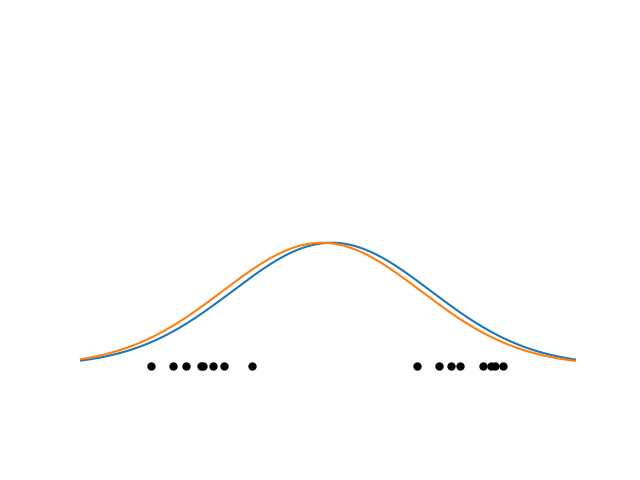
\includegraphics[width=0.45\textwidth]{figures/mixture_bad.png}
%\caption{.}
\vfill
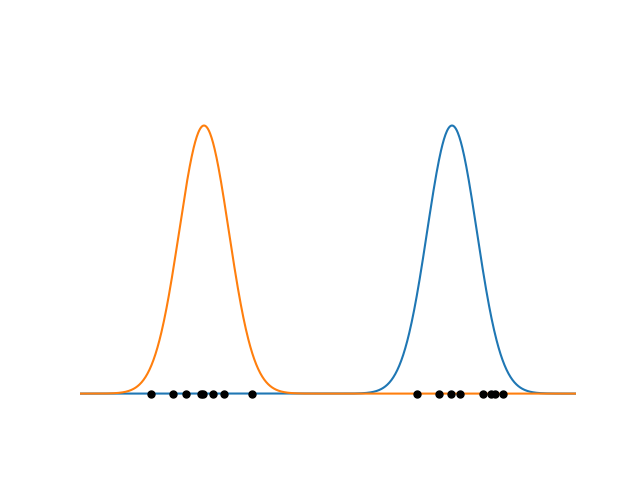
\includegraphics[width=0.45\textwidth]{figures/mixture_good.png}
\caption{\small When sampling from the prior (say, it's a uniform binary code), we end up updating the same class-conditional ${\condprob{p}{}{\x=x}{\z=j}}$ for some $j\in\{1,2\}$ and for all $x$ in the data set. 
Thus, there's no difference between the learned latent code $j$ (top).
If we sample more cleverly by grouping the data points, and assigning larger probability to $p_1(z=j)$ for group 1 and to $p_2$ for group 2, different latent code $j$ will be updated to correspond to a different and sharper class-conditional likelihood ${\condprob{p}{}{\x}{\z=j}}$ (bottom). }
\label{fig:fromprior1}
\end{center}
\end{figure}

\begin{figure}
\begin{center}
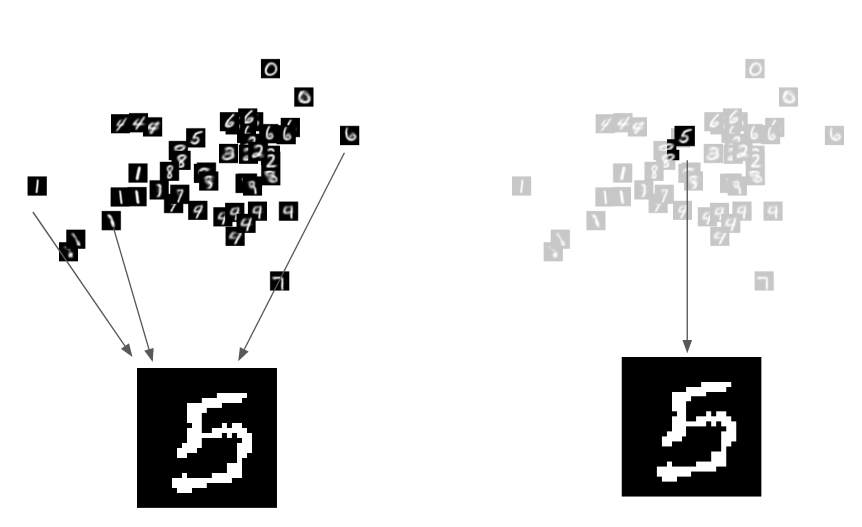
\includegraphics[width=0.85\textwidth]{figures/q_vs_noq.png}
\caption{Left: Sampling from $\prob{p}{}{\x}$, Right: Sampling from $\condprob{q}{}{\x}{\z}$. Using an approximate posterior $q$ narrows down the region in the latent space.}
\label{fig:fromprior2}
\end{center}
\end{figure}
The problem with this approach is that it has \emph{high variance} (see Figure \ref{fig:fromprior1} and \ref{fig:fromprior2}). Think about what we are trying to do here: We have $\x$, and we're trying to maximise $\prob{p}{}{\z}$. However, what the latent variable model is saying is that there is \emph{some} or \emph{several} $\z$s that will generate the observed $\x$. But because we don't know what those $\z$s are, we're just randomly picking out a few from the distribution, pushing them through the generative process, and hoping they hit the mark.

Here's where $q$ comes in to save the day (Yes, just like Star Trek).

We come up with an \emph{approximate posterior}, or in deep learning parlance, an encoder, $\condprob{q}{}{\z}{\x}$. Its job? To \sout{boldly go where} narrow down the area in the prior distribution $\prob{p}{}{\z}$ so that we have an easier time generating something close to the true $\z$ that corresponds to the observed $\x$. 

Now, to relate it back to the information-theoretic point-of-view, narrowing down the search space is akin to giving the model more ``information'' about where in the latent space the corresponding latent state is.

Of course, none of this comes for free. Let's take a look at what introducing $q$ means:
\begin{align*}
\prob{p}{}{\x} 
&= \int \condprob{p}{}{\x}{\z} \prob{p}{}{\z} \mathrm{d}\z \\
&= \int \underbrace{\condprob{q}{}{\z}{\x} \frac{\condprob{p}{}{\x}{\z} \prob{p}{}{\z}}{\condprob{q}{}{\z}{\x}}}_{\text{multiplication by 1!}} \mathrm{d}\z = \expected{\condprob{q}{}{\z}{\x}}{\condprob{p}{}{\x}{\z} 
\frac{\prob{p}{}{\z}}{\condprob{q}{}{\z}{\x}}} 
\end{align*}
Again, we can sample, but this time from $\condprob{q}{}{\z}{\x}$. 
However, notice that the quantity is now weighted by the ratio $\frac{\prob{p}{}{\z}}{\condprob{q}{}{\z}{\x}}$. 

So, if we're trying to maximise $\log \prob{p}{}{\x}$,
\begin{align*}
\log \prob{p}{}{\x} &= 
\log \expected{\condprob{q}{}{\z}{\x}}{
\condprob{p}{}{\x}{\z} \frac{\prob{p}{}{\z}}{\condprob{q}{}{\z}{\x}}} 
\intertext{then, due to Jensen's inequality,}
&\geq \expected{\condprob{q}{}{\z}{\x}}{\log
\condprob{p}{\theta}{\x}{\z} \frac{\prob{p}{\theta}{\z}}{\condprob{q}{\phi}{\z}{\x}}} = \ELBO(\theta, \phi;x) 
\end{align*}
and we get the lower-bound. We use subscripts to denote parameters of the distributions.

The gap between $\log \prob{p}{}{\x}$ and this lower-bound is known as the \emph{variational gap}, and has its own interpretation (Covered in some appendix).\todo{CW: talk about bias in parameter estimate (trade-off of VI versus MCMC)}

\section{The Holy Trinity}

\todo[inline, color=green!40]{Briefly explain what improving each of the following aspects entails.}
If we consider the standard, single-latent-variable model, there are three main pieces we define, and then optimise over:
\begin{itemize}
\item \textbf{The approximate posterior}
$$\condprob{q}{}{\z}{\x} $$
Otherwise called the \emph{encoder}, or the \emph{inference} network in the context of VAEs, where they're parameterised by a deep network (written here as $f$). The conditional distribution over $\z$ given the data $\x$ is usually defined as Gaussian, with parameters that are a function of $\x$, $\condprob{q}{}{\z}{\x} = \N\left(f_\mu(\x), f_\sigma(\x)\right)$.
\item \textbf{The likelihood}
$$\condprob{p}{}{\x}{\z}$$
Otherwise called the \emph{decoder}, or the \emph{generative} network in the context of VAEs, where they're also parameterised by a deep network.
\item \textbf{The prior}
$$\prob{p}{}{\z}$$
In \cite{kingma2013auto}, this is defined $\N(\mathbf{0}, \mathbf{1})$  and not parameterised.
\end{itemize}
All three aspects of the model can be improved, not only at the level of architecture, but in the types of distributions that are assumed for each of them in the model.

\subsection{Better posteriors}

\begin{figure}
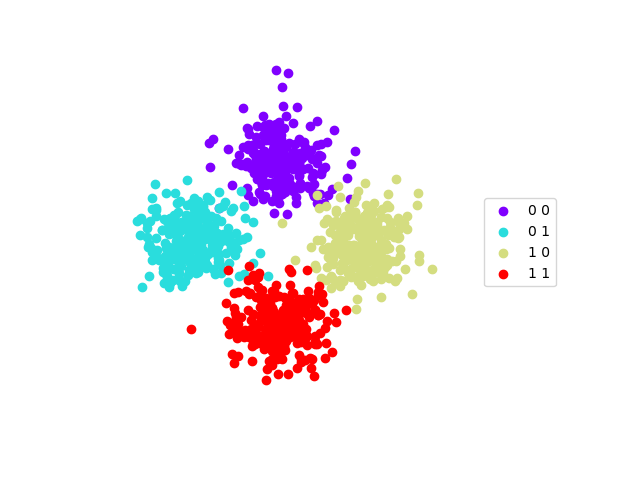
\includegraphics[width=0.5\textwidth]{figures/2bits_gaussian.png}
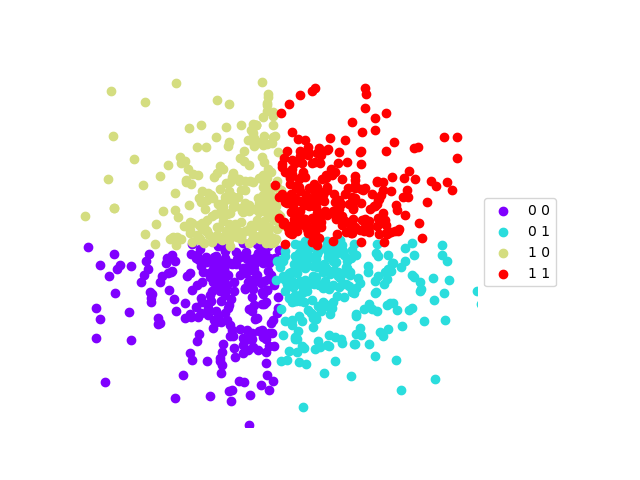
\includegraphics[width=0.5\textwidth]{figures/2bits_dsf.png}
\label{ref:gauss_vs_flow}
\caption{Left: Gaussian approximate posterior, Right: Non-gaussian aproximate posterior.}
\end{figure}

Recall again that one of the goals of the generative model is to allow us to sample from the distribution over $\z$, and generate reasonable examples of our data. Ideally, this also means that there has to be a mapping from the data $\x$ to the distribution over $\z$ such that marginalising out the data, we recover the defined prior over $\z$.

Unfortunately, defining the approximate posterior as a Gaussian may not satisfy this requirement well enough. 
Consider a two-bit example: we sample $(x_a,x_b)$ from two independent Bernoulli distributions both with probability being $0.5$.
There are four possibilities. 
And we want to learn a VAE on this dataset.
If we assume the approximate posteriors to be Gaussians (see left of Figure \ref{ref:gauss_vs_flow}), then we would end up with an aggregate posterior $q(z) = \sum_{i=1}^4 q(z_i|x_i)\tilde{p}(x_i)$ being a mixture of Gaussians that fails to be prior-like ($p(z)=\N(z;0,I)$ in this case). 
This is because the posterior distributions fail to capture the true ones, and if our inference network $q(z|x)$ is good enough to perfectly model the true posteriors, the aggregate posteriors should be the shape of the prior (see right of Figure \ref{ref:gauss_vs_flow}) \footnote{See \cite{hoffman2016elbo} or \cite{huang2017led} for the derivation}.

Turns out, the easiest remedy to this is to have a better posterior. 
With a bit of rearrangement and the introduction of a few new notations, the variational gap can be divided into the following three parts:
\begin{equation}
\begin{split}
\log p_{\theta}(x) - &\ELBO(\theta, \phi; x) = \\
&\underset{\text{Gap 1}}{\underbrace{\KL{q^*}{p}}} + \underset{\text{Gap 2}}{\underbrace{[\KL{q^*_\theta}{p}-\KL{q^*}{p}]}} + \underset{\text{Gap 3}}{\underbrace{[\KL{q_\theta}{p}-\KL{q^*_\theta}{p}]}}
\end{split}
\end{equation}
where  
\begin{itemize}
\item $p$ is the true posterior
\item $q^*$ is the optimal approximate posterior within the family $\mathcal{Q}=\{q\in \mathcal{Q}\}$
\item $q^*_\phi$ is the optimal approximate posterior within the family $\mathcal{Q}_\phi\subseteq\mathcal{Q}$ due to the amortized inference via the conditional mapping $\phi\in\Phi:x\rightarrow \pi_q(x;\phi)$ where $\pi_q$ denotes the parameters of distribution $q$, and finally
\item $q_\phi$ is the approximate posterior that we are analyzing. 
\end{itemize}


The first gap and the combination of Gap 2 and Gap 3 are what \citet{cremer2017inference} called \textit{approximation gap} and \textit{amortization gap}. 
With these, we know that there are three pieces to improve in order to make the variational gap smaller:

\begin{enumerate}
\item better $\mathcal{Q}$, i.e. the choice of family of distributions. This can be achieved by choosing a larger family of distributions (such as normalizing flows).
\item better $\Phi$, i.e. better amortized inference. This can be achieved by having a higher capacity encoder.
\item better $\phi$, i.e. better encoder within the family $\Phi$. This can be achieved by improving the optimization scheme. 
\end{enumerate}

In Table \ref{tb:betterpos} we list a few approaches designed to improve variational inference by making the variational gap smaller. 

\begin{table}
\caption{Methods that aim at reducing the variational gap.}
\label{tb:betterpos}
\centering
\begin{tabular}{lccc}
\toprule
& Gap 1 & Gap 2 & Gap 3 \\
\midrule
Better optimization &&&\xmark\\
Better encoder \cite{cremer2017inference}&&\xmark&\\
Normalizing flows \cite{rezende2015variational,kingma2016improving,huang2017facilitating} &\xmark&&\\
Hierarchical VI \cite{ranganath2016hierarchical,maaloe2016auxiliary}&\xmark&&\\
Implicit VI \cite{mescheder2017adversarial,huszar2017variational}&\xmark&&\\
Variational boosting \cite{miller2016variational}&\xmark&&\\
MCMC as part of $q_\phi$ \cite{salimans2015markov}&\xmark&&\\
MCMC on top of $q_\phi$ \cite{de2001variational,hoffman2017learning} &\xmark&\xmark&\xmark\\
Gradient flow \cite{duvenaud2016early} &\xmark&\xmark&\xmark\\
Importance sampling \cite{burda2015importance}&\xmark&\xmark&\xmark\\
\bottomrule
\end{tabular}
\end{table}



\subsection{Better likelihood}
Consider modelling an image using a single latent variable model. In order to produce a reasonable, realistic looking image, we need to decide the objects in the image, their location, abstract stuff. But beyond these abstract ideas, there are also the details, like lighting and texture that we need to model. 

When the probability of the given datapoint is defined as being factorised over every dimension, the implication is that the distribution over the observation \todo{CW: or the correlation between the observed variables depends on ...; cos marginal independency could also be a model assumption} is completely dependent upon the latent variable. However, the latent variable has limited capacity, and may model only the aspects that contribute to most of the reconstruction loss (abstract concepts) and there may be variations at a lower level of abstraction that may depend on other parts of the input (details).

\todo{CW: be more general}Modelling the data this way are what we'll call autoregressive generative models, and some examples of such models are \cite{gulrajani2016pixelvae} for images, with a slightly more general discussion found in \cite{chen2016variational}, and \cite{bowman2015generating} for text. 

\todo{CW: missing VAE w/o pixelwise reconstruction}


\subsection{Better priors}

\begin{figure}
\centering
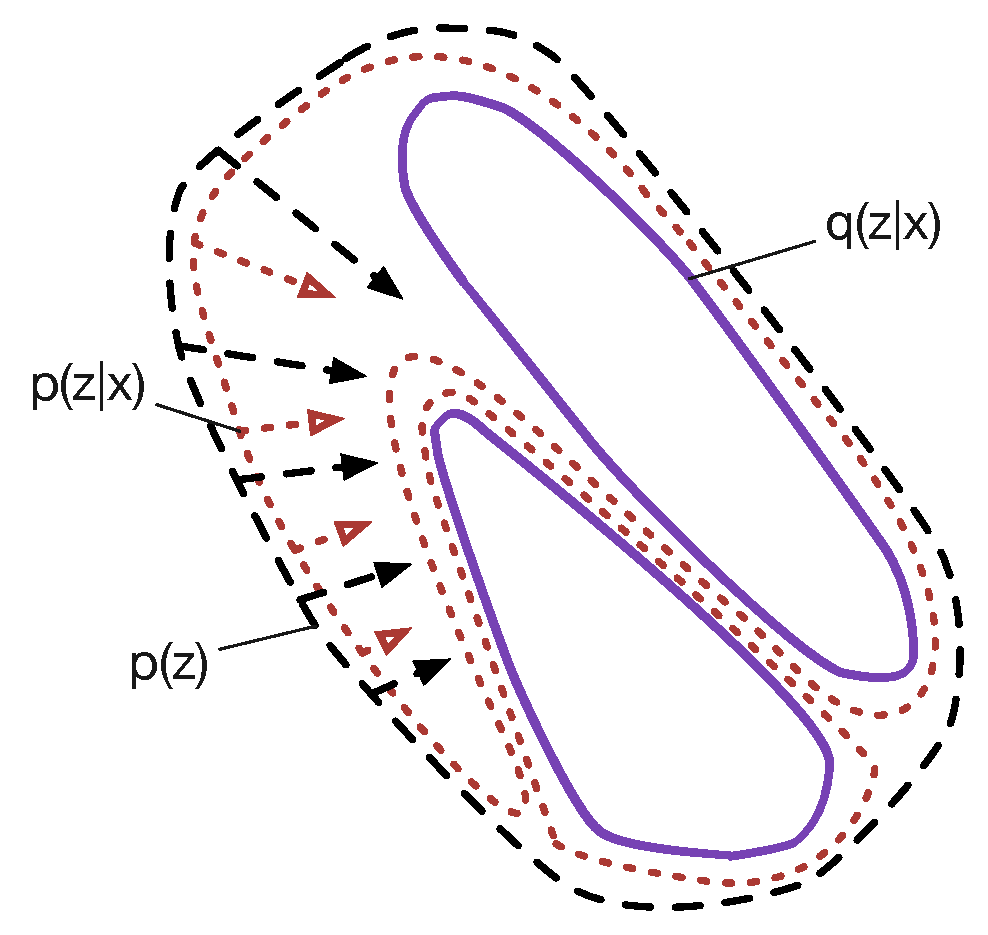
\includegraphics[width=0.5\textwidth]{figures/mmp.pdf}
\label{ref:mmp}
\caption{}
\end{figure}

Just as we can modify the approximate posterior to fit the prior better, we can also modify the prior such that it is learned from the data.

The expressivity of neural networks and developments in improving the posteriors allow the data to be mapped really well to simple priors like a Gaussian. So if we can already modify the posterior, why bother changing the prior? One reason may be due to discontinuity when interpolating in the latent space. Refer again to Figure \ref{ref:gauss_vs_flow}. If we imagine each colour code to be a different modality in the data, moving from one colour group to another will represent a drastic change in the type of data decoded\todo{CW: talk about inductive bias}. This means that sampling from close regions in the latent space may not represent close relationships in the data space. Allowing the prior to model a lower density between these different modalities may be more ideal when the type of representation learned is more important than simply sampling data points from the model.

\cite{tomczak2017vae} proposes parameterising the prior as a mixture over a sample of the dataset, or using learned \emph{pseudo-inputs}. \cite{serban2016multi} introduces a prior parameterised by a piece-wise linear function. In \cite{huang2017led}, the authors parameterise the prior with Real NVP transformations \citep{dinh2016density}.

\section{Evaluating the model}
Depending on what your metric of model ``goodness'' is, there may be different ways to evaluate a given model. Some may care about disentanglement of factors in the latent variable, while others may care more about generating realistic looking images\footnote{VAEs do poorly at this... for now. (circa Jan 2018)}. In this article, we discuss evaluation in terms of estimating the probability density defined by the model for a given datapoint.

While we may train the model using the VLB, we need to evaluate $\log \prob{p}{}{\x}$. The procedure for doing this is simply importance sampling, as described in the previous section,
\begin{align*}
\log \prob{p}{}{\x} &= 
\log \expected{\condprob{q}{}{\z}{\x}}{
\condprob{p}{}{\x}{\z} \frac{\prob{p}{}{\z}}{\condprob{q}{}{\z}{\x}}} \\
&\approx \log \sum_{k=1}^K 
\condprob{p}{}{\x}{\z} \frac{\prob{p}{}{\z_k}}{\condprob{q}{}{\z_k}{\x}}, &\z_k \sim \condprob{q}{}{\z}{\x}
\end{align*}
However, as with most instances in machine learning, the probabilities are computed in log space,
\begin{align*}
&\log \sum_{k=1}^K 
\condprob{p}{}{\x}{\z} \frac{\prob{p}{}{\z_k}}{\condprob{q}{}{\z_k}{\x}} =\\
&\qquad \underbrace{\log \sum_{k=1}^K \exp}_\text{There's a trick for that}\left(
\log \condprob{p}{}{\x}{\z} + \log \prob{p}{}{\z_k} - \log \condprob{q}{}{\z_k}{\x}
\right)
\end{align*}
And we can use the $\mathrm{logsumexp}$ trick to deal with that sum over the probabilities. This has been mentioned in and \cite{rezende2014stochastic} Appendix E.

 \cite{kingma2013auto} Appendix D, 

\section{How to Train your VAE}
The purpose of this section is to explicitly introduce what various key papers on VAEs have demonstrated about modelling data or training using VAEs. 
\todo[inline, color=green!40]{clearly needs a rewrite lol.}

\begin{enumerate}
\item Design the graphical model,
\item Decide the types of distributions over the different variables,
\item Make some simplifying assumptions if it's too complicated,
\end{enumerate}
\subsection{Semi-supervised settings}
%\cite{kingma2014semi} introduces a way to model partially labelled data with variational autoencoders. Specifically in the setting they used, the data was MNIST\footnote{because everything works on MNIST} and SVHN. The observed data are the images, while the labels are only partially observed: sometimes you have them, sometimes you don't.

%Naturally, the thing to do in this situation is to marginalise over all possible labels. In this scenario, since there are only 10 digits, this is possible. When the number of classes gets large, perhaps sampling might be in order. However, there are tradeoffs involved when dealing with discrete variables, for more information see the subsection about discrete variables.

\todo[inline, color=green!40]{``how'' more in details}

The partially available data need not be a discrete variable, like a label. It could be parts of the data which are missing in some parts of the dataset, and making a prediction requires doing some form of \emph{imputation} over the missing random variables. For conditional distributions of such missing data that have distributions you can sample from during training, the same reparameterisation trick can be applied.


\subsection{Hierarchy of Latent Variables}
For modeling images, it might be useful to model noise at different abstractions of the generation process. One way to view this generation process may be a hierarchy of latent variables, starting at the highest level of abstraction $z_L$, down to the lowest $z_1$.
Consider a VAE with an inference model $q$,
$$q(z_1, z_2,\dots,z_L | x) = q(z_1|x)q(z_2|z_1) \dots q(z_L|z_{L-1})$$
and generative model,
$$p(x|z_1, z_2,\dots,z_L) = p(z_L) p(z_{L-1}|z_L)\dots p(z_1|z_2)p(x|z_1) $$

One interesting thing to note is that the resulting loss for such a model (where the generative model is not autoregressive), is that the reconstruction loss (at the bottom) never directly backpropagates gradients to the higher layers.
\todo[inline, color=green!40]{Incomplete... cite \cite{sonderby2016ladder}}

\begin{align*}
&\expected{\condprob{q}{\phi}{z_1,\hdots,z_L}{x}}{\log p(x|z_1)} \\
&\qquad  - \expected{\condprob{q}{\phi}{z_1,\hdots,z_L}{x}}{\log \condprob{q}{\phi}{z_1,\hdots,z_L}{x} - 
 \log \prob{p}{\theta}{z_1,\hdots,z_L}
} \\
 &= \mathbb{E}_{\condprob{q}{\phi}{z_1}{x}}\left[{\log p(x|z_1)}\right. \\
&\qquad
	- \mathbb{E}_{\condprob{q}{\phi}{z_2}{z_1}}\left[
  	\log \condprob{q}{\phi}{z_1}{x} - 
 	\log \condprob{p}{\theta}{z_1}{z_2}\right.
\\
&\qquad\qquad\left.\left.
	- \mathbb{E}_{\condprob{q}{\phi}{z_3}{z_2}}\left[
  	\log \condprob{q}{\phi}{z_2}{z_1} - 
 	\log \condprob{p}{\theta}{z_2}{z_3} \hdots \right]\right]\right]
\\
 &\approx \expected{\condprob{q}{\phi}{z_1}{x}}{\log p(x|z_1)} \\
&\qquad - \KL{\condprob{q}{\phi}{z_1}{x}}{\condprob{p}{\theta}{z_1}{z_2}} \\
&\qquad - \KL{\condprob{q}{\phi}{z_L}{z_{L-1}}}{\prob{p}{}{z_L}} \\
&\qquad - \sum^{L-1}_{l=2} \KL{\condprob{q}{\phi}{z_l}{z_{l-1}}}{\condprob{p}{\theta}{z_l}{z_{l+1}}}
\end{align*}
As seen in the derivation, the reconstruction term uses only $z_1$, the first latent variable in the hierarchy, the subsequent layers are optimised by the KL-divergence terms.

\subsection{Discrete variables}
\todo{CW: talk about why we care about discrete latent variables (motivations!)}One option to deal with discrete latent variables is by replacing it with a continuous distribution that's ``close enough'' to the discrete distribution. Both \cite{maddison2016concrete} and \cite{jang2016categorical} introduce a relaxation of the discrete distributions using the Gumbel distribution, which a similar reparameterisation trick can be used in order to sample from it.

Another option is to sample from the distribution, and estimate the gradient during backpropagation. Some options are the straight-through estimator \citep{bengio2013estimating}, and REINFORCE \citep{williams1988use}.

\subsection{Sequential data}
\todo{cW: motivations! [note: probably more on the ambiguity of language, for example]}There has been some work that deals with sequential data using VAEs. \cite{chung2015recurrent} incorporates latent variables into an RNN. One thing to highlight here is the possibility of conditioning the prior of the latent variable on past, seen, data.

In \cite{shabanian2017variational}, the approximate posterior is conditioned on the entire sequence. This makes sense since if $\z_t$ is responsible for the observation $\x_t$, and $\z_t$ is dependent on the \emph{previous} time step's latent variable $\z_{t-1}$, then $\z_t$ is conditionally dependent on the entire sequence. The resulting model can still be used as a generative model to generate sequence, despite the approximate posterior being conditioned on the full $\x$.

\subsection{Strong Decoders}
\todo{CW: refer to the ``high level semantics'' part}In some autoregressive models, it may be possible for the generative model to ignore the latent variable. Examples of such models are language models conditioned on a latent variable \citep{bowman2015generating}, and PixelVAEs \citep{gulrajani2016pixelvae}. Because the models already work relatively well without the global information provided by the latent variable, the KL-divergence term goes to 0.

One quick remedy for this is to set an annealing term $\beta$ for the KL-divergence term,
$$\expected{\condprob{q}{}{\z}{\x}}{\log \condprob{p}{}{\x}{\z}}
- \beta \cdot \KL{\condprob{q}{}{\z}{\x}}{\log \prob{p}{}{\z}}.$$
This has been given some theoretical justification in \cite{higgins2016beta} and \cite{alemi2017information}, where interpretations of $\beta$ are given.

Another possibility is to ``weaken'' the generative model. For example, in \cite{yang2017improved}, instead of an RNN for text generation, they used a CNN for the decoder.
\todo{CW: missing free bits (ref:iaf)}

\subsection{Wherever possible, reduce variance}
\todo{CW: this is what VI is about (smaller variance but biased!); link to Max welling's DL summer school talk }One of the core motivations for the contributions in \cite{kingma2013auto} was methods for variance reduction. Whenever sampling is performed, variance is introduced. Before, methods for backpropagating through random samples involved gradient estimates, like \cite{williams1988use}, \cite{bonnet1964transformations} and \cite{price1958useful} \footnote{As you can see, these go pretty far back.}. The issue with these gradient estimates is usually high variance. The reparameterisation trick ameliorates the problem as the variance is bounded by a constant (More details can be found in the appendix of \cite{rezende2014stochastic}.)

%CW: I would prefer to talk about this in the training part (variance reduction section). Here it feels more natural to talk about what this ``view'' means (compared to the information theoretic one) and what these terms mean.
% Shawn: I think as far as most practitioners are concerned, training mostly means actually training it and less about worrying about variance and such, but I agree it's probably more appropriate there.
Recall in the previous explanation about the ELBO that the entire purpose of introducing $q$ in training is variance reduction. 
Given that we are using SGD as our training method,
%CW: sgd is another independent source of noise yeah
%ST: Yeah isn't that part of the reason why we need to reduce variance
the importance of doing this cannot be understated.

We \emph{may} still be able to further reduce variance during training if we are able to analytically compute parts of the terms in this lower-bound. Notice, 
\begin{align*}
\expected{\condprob{q}{}{\z}{\x}}{\log
\condprob{p}{}{\x}{\z} \frac{\prob{p}{}{\z}}{\condprob{q}{}{\z}{\x}}} 
&= \expected{\condprob{q}{}{\z}{\x}}{\log \condprob{p}{}{\x}{\z}} + 
\underbrace{\expected{\condprob{q}{}{\z}{\x}}{\log \frac{\prob{p}{}{\z}}{\condprob{q}{}{\z}{\x}}}}_{\text{Look familiar?}} \\
&= \expected{\condprob{q}{}{\z}{\x}}{\log \condprob{p}{}{\x}{\z}} - 
\underbrace{\expected{\condprob{q}{}{\z}{\x}}{\log \frac{\condprob{q}{}{\z}{\x}}{\prob{p}{}{\z}}}}_{\text{What about now?}} \\
&= \expected{\condprob{q}{}{\z}{\x}}{\log \condprob{p}{}{\x}{\z}} - 
\KL{\condprob{q}{}{\z}{\x}}{\log \prob{p}{}{\z}}
\end{align*}
If both $\condprob{q}{}{\z}{\x}$ and $ \prob{p}{}{\z}$ are parameterised as Gaussians, for example, as they are in the original VAE paper, then there is a closed form for this KL-Divergence term.

\todo{CW: missing new paper ``Reducing Reparameterization Gradient Variance'' by miller NIPS2017}

\appendix
\section{More derivations}
\begin{align*}
\log \prob{p}{}{\x} 
&=  \log \int \condprob{p}{}{\x}{\z} \prob{p}{}{\z} \mathrm{d}\z \\
&= \log \int \condprob{q}{}{\z}{\x} \frac{\condprob{p}{}{\x}{\z} \prob{p}{}{\z}}{\condprob{q}{}{\x}{\z}} \mathrm{d}\z \\
&= \log \expected{\condprob{q}{}{\z}{\x}}{
\frac{\condprob{p}{}{\x}{\z} \prob{p}{}{\z}}{\condprob{q}{}{\z}{\x}}} \\
&\geq \expected{\condprob{q}{}{\z}{\x}}{\log 
\frac{\condprob{p}{}{\x}{\z} \prob{p}{}{\z}}{\condprob{q}{}{\z}{\x}}} \\
&= \expected{\condprob{q}{}{\z}{\x}}{\log \condprob{p}{}{\x}{\z}} - \KL{\condprob{q}{}{\z}{\x}}{\prob{p}{}{\z}}
\end{align*}

\begin{align*}
\KL{\condprob{q}{}{\z}{\x}}{\condprob{p}{}{\z}{\x}}
&= \expected{\condprob{q}{}{\z}{\x}}{\log 
\frac{\condprob{q}{}{\z}{\x} }{\condprob{p}{}{\z}{\x}}} \\
&= \expected{\condprob{q}{}{\z}{\x}}{
 	\log \condprob{q}{}{\z}{\x} 
 	\frac{\prob{p}{}{\x}}{\condprob{p}{}{\x}{\z} \prob{p}{}{\z}}} \\
&= \expected{\condprob{q}{}{\z}{\x}}{
 	\log \frac{\condprob{q}{}{\z}{\x}}{\prob{p}{}{\z}} 
 	\frac{\prob{p}{}{\x}}{\condprob{p}{}{\x}{\z}}} \\
&=\expected{\condprob{q}{}{\z}{\x}}{
 	\log \frac{\condprob{q}{}{\z}{\x}}{\prob{p}{}{\z}}} -
   \expected{\condprob{q}{}{\z}{\x}}{\log \condprob{p}{}{\x}{\z}} + \log \prob{p}{}{\x} \\
\log \prob{p}{}{\x} -
\underbrace{\KL{\condprob{q}{}{\z}{\x}}{\condprob{p}{}{\z}{\x}}}_{
	\text{Variational gap}
}
&= \expected{\condprob{q}{}{\z}{\x}}{\log \condprob{p}{}{\x}{\z}} - \KL{\condprob{q}{}{\z}{\x}}{\prob{p}{}{\z}}	
\end{align*}



\paragraph{Glossary}

\begin{itemize}
\item VAE: variational autoencoder
\item DLGM: deep latent gaussian model
\item LVM: latent variable model
\item DNN: deep neural networks
\end{itemize}

\paragraph{Notation}
\begin{itemize}
\item $\tilde{p}$: unknown distribution
\item $\expected{x\sim p(x)}{f(x)}=\int_x p(x)f(x)dx$: expected value of $f(x)$, a deterministic feature of $x$, under the distribution $p(x)$
\item $\KL{\prob{q}{}{x}}{\prob{p}{}{x}} = \int_x q(x)\log\frac{q(x)}{p(x)}$: KL divergence between $q$ and $p$
\end{itemize}

\bibliography{bib} 
\bibliographystyle{plainnat}
\end{document}






